

\section*{K5/4. feladat: Hengeres fal közelítése síkfallal}
\addcontentsline{toc}{section}{K5/4. feladat: Hengeres fal közelítése síkfallal}

\begin{tabular}{ | p{2cm} | p{14cm} | } 
	\hline
	Név & Szalay István \\ 
	\hline
	Szak & \\ 
	\hline
	Félév & 2019/2020 II. (tavaszi) félév \\ 
	\hline
\end{tabular}
\vspace{0.5cm}

\noindent Gyakorlati számítások során szokás a hengeres falon vezetéssel átjutó hőáramot közelítő módon síkfalra vonatkozó összefüggésekkel számolni. Határozza meg egy hengeres fal külső $d_2$ és belső $d_1$ átmérőjének hányadosa függvényében, hogy a lineáris hőáramsűrűség számításakor hány \%-os hibát vétünk az alábbi közelítő összefüggéseket használva:
\begin{equation}
	\dot{q}_{lin} = \dfrac{\lambda}{\delta} d_K \pi \left(T_1 - T_2\right),
	\quad 
	\delta = \dfrac{d_2 - d_1}{2}, 
	\quad 
	\text{és} 
	\quad d_K = \dfrac{d_1 + d_2}{2}
\end{equation}

ahol $\delta$ a falvastagság és $d_K$ a közepes átmérő.


\begin{figure}[h]
	\centering
	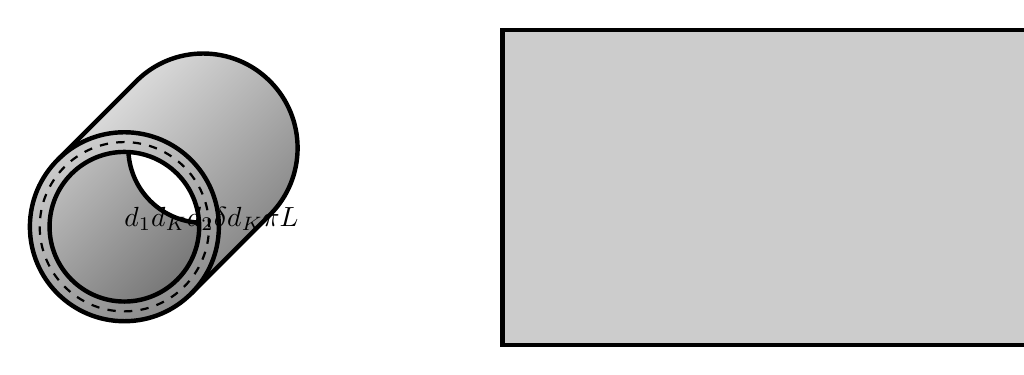
\begin{tikzpicture}
		\pgfmathsetmacro{\DB}{1.9}
		\pgfmathsetmacro{\DK}{2.4}
		
		\shade[shading=axis, bottom color=black!20, top color=black!60, shading angle=-135, even odd rule] (0,0) circle[radius=\DB/2] (1, 1) circle[radius=\DB/2];
		\draw[ultra thick] (1, 1) circle[radius=\DB/2];
		
		\shade[shading=axis, bottom color=black!10, top color=black!50, shading angle=-135] ({-\DK/2/sqrt(2)}, {\DK/2/sqrt(2)}) arc [start angle=135, end angle=-45, radius={\DK/2}] -- ({1+\DK/2/sqrt(2)}, {1-\DK/2/sqrt(2)}) arc [start angle=-45, end angle=135, radius={\DK/2}] -- cycle;
		
		\shade[shading=axis, bottom color=black!20, top color=black!45, shading angle=-150, even odd rule] (0,0) circle[radius=\DK/2] circle[radius=\DB/2];
		
		\draw[ultra thick] ({-\DK/2/sqrt(2)}, {\DK/2/sqrt(2)}) -- ({1-\DK/2/sqrt(2)}, {1+\DK/2/sqrt(2)}) arc [start angle=135, end angle=-45, radius={\DK/2}] -- ({\DK/2/sqrt(2)}, {-\DK/2/sqrt(2)});
		
		\draw[ultra thick] (0, 0) circle[radius=\DB/2];
		\draw[ultra thick] (0, 0) circle[radius=\DK/2];
		\draw[thick, dashed] (0, 0) circle[radius={(\DB+\DK)/4}];
		
		\pgflength[xa=-\DB/2, ya=0, xb=\DB/2, yb=0, ra=\DK/2+0.6]{$d_1$};
		\pgflength[xa={-\DB/4-\DK/4}, ya=0, xb={\DB/4+\DK/4}, yb=0, ra=\DK/2+1.2]{$d_K$};
		\pgflength[xa=-\DK/2, ya=0, xb=\DK/2, yb=0, ra=\DK/2+1.8]{$d_2$};
		
		\pgflength[xa=-\DK/2, ya=0, xb=-\DB/2, yb=0, ra=-\DK/2-0.5, belül=2]{$\delta$};
		
		\draw[ultra thick, fill=black!20] (3.5, -1.5) rectangle ({3.5+\DK*3.14},{2.5});
		\pgflength[xa=3.5, ya=-1.5, xb={3.5+\DK*3.14}, yb=-1.5]{$d_K \pi$};
		\pgflength[xa={3.5+\DK*3.14}, ya=-1.5, xb={3.5+\DK*3.14}, yb=2.5]{$L$};
		
	\end{tikzpicture}
	\caption{Hengeres fal kiterítése és közelítése síkfallal.}
\end{figure}

A hőáramra vonatkozó valós és a közelítő összefüggés:
\begin{equation}
	\dot{Q}_{\textit{valós}} = \dfrac{2 \pi \lambda L}{\ln\frac{d_2}{d_1}} \left(T_1 - T_2\right) 
	\quad \textrm{és} \quad 
	\dot{Q}_{\textit{közelítő}} = \dfrac{2 \lambda}{d_2 - d_1} \dfrac{d_1 + d_2}{2} \pi L\left(T_1 - T_2\right)
\end{equation}

A vizsgálatot a $\varphi = \dfrac{d_2}{d_1} \in \left[1, 3\right]$ intervallumban, 0,5-es lépésekben végezzük el. A vizsgálat az $\varepsilon$ relatív hiba értékének kiszámítását jelenti a $\varphi$ átmérőhányados különböző értékei mellett. A relatív hiba, behelyettesítve a hőáramokat:
\vspace{-2mm}
\begin{equation}
	\varepsilon = \dfrac{\dot{Q}_{\textit{valós}} - \dot{Q}_{\textit{közelítő}}}{\dot{Q}_{\textit{valós}}} = 1 - \dfrac{\dot{Q}_{\textit{közelítő}}}{\dot{Q}_{\textit{valós}}} = 
	1 - \dfrac{
		\dfrac{\bcancel{2} \bcancel{\lambda}}{d_2 - d_1} \dfrac{d_1 + d_2}{2} \bcancel{\pi} \bcancel{L} \cancel{\left(T_1 - T_2\right)}
	}{
		\dfrac{\bcancel{2} \bcancel{\pi} \bcancel{\lambda} \bcancel{L}}{\ln\frac{d_2}{d_1}} \cancel{\left(T_1 - T_2\right)}
	}
\end{equation}

Kifejezve $d_2$-t $\varphi d_1$ alakban:
\begin{equation}
	\varepsilon = 
	1 - \dfrac{d_1 + d_2}{d_2 - d_1} \dfrac{1}{2} \ln\frac{d_2}{d_1} = 
	1 - \dfrac{d_1 + \varphi d_1}{\varphi d_1 - d_1} \dfrac{1}{2} \ln\varphi = 
	1 - \dfrac{1 + \varphi}{\varphi - 1} \dfrac{1}{2} \ln\varphi
\end{equation}

A relatív hiba értékei a vizsgált intervallumban:

\begin{table}[h!]
	\centering
	{\tabulinesep=1.2mm
		\begin{tabu} {|l |[1.5pt] c | c | c | c | c|}
			\hline
			$\varphi$ & 1 & 1,5 & 2 & 2,5 & 3
			\\ \tabucline [1.5pt]{-}
			$\varepsilon\!\left(\varphi\right)$ & 
			$\displaystyle \lim_{\varphi\to 1+} \varepsilon\!\left(\varphi\right) = 0$ &
				0,0134 & 
				0,0382 & 
				0,0645 & 
				0,0897
			\\ \hline
		\end{tabu}
	}
\end{table}

\pagebreak
